\documentclass{ctexart}
\usepackage{amsmath}
\usepackage{amssymb}
\usepackage{amsthm}
\usepackage{graphicx}
%\usepackage{multirow}
\usepackage{tikz}
\usetikzlibrary{arrows,decorations.pathmorphing,backgrounds,positioning,fit}
\usetikzlibrary{calc,through,backgrounds}
\usepackage[numbers]{natbib}
\author{付乃锋}
\title{广义相对论下N体问题的一阶近似}
\date{\today}
\begin{document}
\maketitle
%\tableofcontents
\begin{abstract}
\par 众所周知,天文学研究已历经几千年,
催生出了许许多多数学及物理知识与与应用,
自伽利略、牛顿以来,是构建经典物理学体系的先导。
如今,现代物理学研究中,天文学中的N体问题依然没有获得解析解,
依然是新的物理理论的检验方式,新的数学知识的应用天地。自上世纪初,
爱因斯坦提出狭义相对论与广义相对论,天文学的研究进入了新的阶段,
相对论已经广泛应用于卫星控制及天体观测等方面,
特别是GPS应用中授时与精确定位等方面相对论效应改正。
本文探讨的是广义相对论下N体问题的一阶近似问题,
又称为一阶后牛顿近似。
\par \textbf{Keywords:} Einstain-field-function,DXS
\end{abstract}
\section{Introduction}

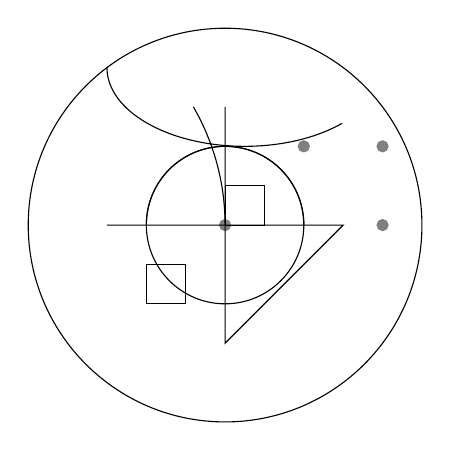
\begin{tikzpicture}
\clip[draw] (0,0) circle (2.5cm);
\filldraw [gray] (0,0) circle (2pt)
(1,1) circle (2pt)
(2,1) circle (2pt)
(2,0) circle (2pt);
%\draw (0,0) .. controls (1,1) and (2,1) .. (2,0);
\draw (-1.5,0) -- (1.5,0) -- (0,-1.5) -- (0,1.5);

\draw (-1,0) .. controls (-1,0.555) and (-0.555,1) .. (0,1)
.. controls (0.555,1) and (1,0.555) .. (1,0);
\draw (0,0) circle (1cm);
\draw (0,0) rectangle (0.5,0.5);
\draw (-0.5,-0.5) rectangle (-1,-1);
\draw (0mm,0mm) arc (0:30:3cm);
\draw (2cm,2cm) arc (0:315:1.75cm and 1cm);
\end{tikzpicture}

\begin{tikzpicture}[rounded corners,ultra thick]
\shade[top color=yellow,bottom color=black] (0,0) rectangle +(2,1);
\shade[left color=yellow,right color=black] (3,0) rectangle +(2,1);
\shadedraw[inner color=yellow,outer color=black,draw=yellow] (6,0) rectangle +(2,1);
\shade[ball color=green] (9,.5) circle (.5cm);
\end{tikzpicture}
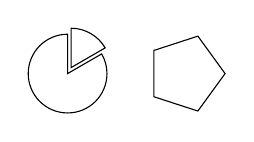
\begin{tikzpicture}[scale=0.5]
\draw (0,0) -- (90:1cm) arc (90:360:1cm) arc (0:30:1cm) -- cycle;
\draw (60:5pt) -- +(30:1cm) arc (30:90:1cm) -- cycle;
\draw (3,0) +(0:1cm) -- +(72:1cm) -- +(144:1cm) -- +(216:1cm) --
+(288:1cm) -- cycle;
\end{tikzpicture}

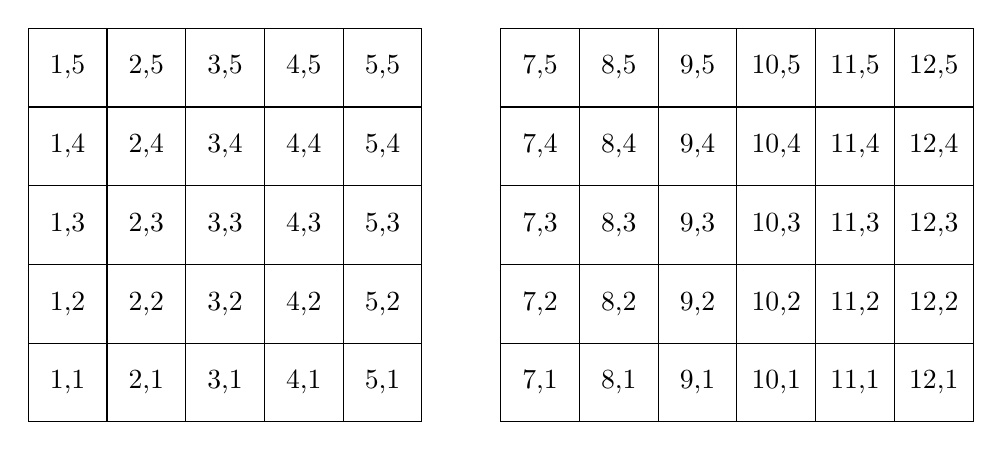
\begin{tikzpicture}
\foreach \x in {1,2,...,5,7,8,...,12}
\foreach \y in {1,...,5}
{
\draw (\x,\y) +(-.5,-.5) rectangle ++(.5,.5);
\draw (\x,\y) node{\x,\y};
}
\end{tikzpicture}

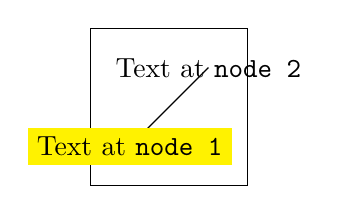
\begin{tikzpicture}
\draw (0,0) rectangle (2,2);
\draw (0.5,0.5) node [fill=yellow]
{Text at \verb!node 1!}
-- (1.5,1.5) node {Text at \verb!node 2!};
\end{tikzpicture}


\par 广义相对论建立在引力和惯性力等效的原理上,
它告诉我们一个任意的物理系统对于外界引力场将作何反应,
具体可以表述为:在任意引力场里的每一个时空点,
有可能选择一个"局部惯性系",使得所讨论的那一点附近的邻域内,
自然规律的形式,与没有引力场时在未加速的Descartes坐标系里具有相同的形式,
即在时空的任一点,我们可以建立一个使物质满足狭义相对论规律的局部惯性系。
如上为强等效原理描述,认为引力质量支配引力对所有物理系统的效应;
弱等效原理,则只表明自然规律仅指"自由降落的质点的运动规律",
即表明引力质量与惯性质量等价。
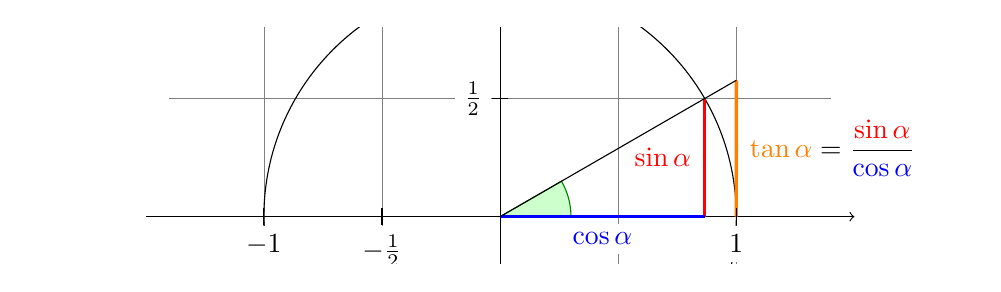
\begin{tikzpicture}[scale=3]
\clip (-2,-0.2) rectangle (2,0.8);
\draw[step=.5cm,gray,very thin] (-1.4,-1.4) grid (1.4,1.4);
\filldraw[fill=green!20,draw=green!50!black] (0,0) -- (3mm,0mm) arc
(0:30:3mm) -- cycle;
\draw[->] (-1.5,0) -- (1.5,0) coordinate (x axis);
\draw[->] (0,-1.5) -- (0,1.5) coordinate (y axis);
\draw (0,0) circle (1cm);
\draw[very thick,red]
(30:1cm) -- node[left=1pt,fill=white] {$\sin \alpha$} (30:1cm |- x axis);
\draw[very thick,blue]
(30:1cm |- x axis) -- node[below=2pt,fill=white] {$\cos \alpha$} (0,0);
\draw[very thick,orange] (1,0) -- node [right=1pt,fill=white]
{$\displaystyle \tan \alpha \color{black}=
\frac{{\color{red}\sin \alpha}}{\color{blue}\cos \alpha}$}
(intersection of 0,0--30:1cm and 1,0--1,1) coordinate (t);
\draw (0,0) -- (t);
\foreach \x/\xtext in {-1, -0.5/-\frac{1}{2}, 1}
\draw (\x cm,1pt) -- (\x cm,-1pt) node[anchor=north,fill=white] {$\xtext$};
\foreach \y/\ytext in {-1, -0.5/-\frac{1}{2}, 0.5/\frac{1}{2}, 1}
\draw (1pt,\y cm) -- (-1pt,\y cm) node[anchor=east,fill=white] {$\ytext$};
\end{tikzpicture}

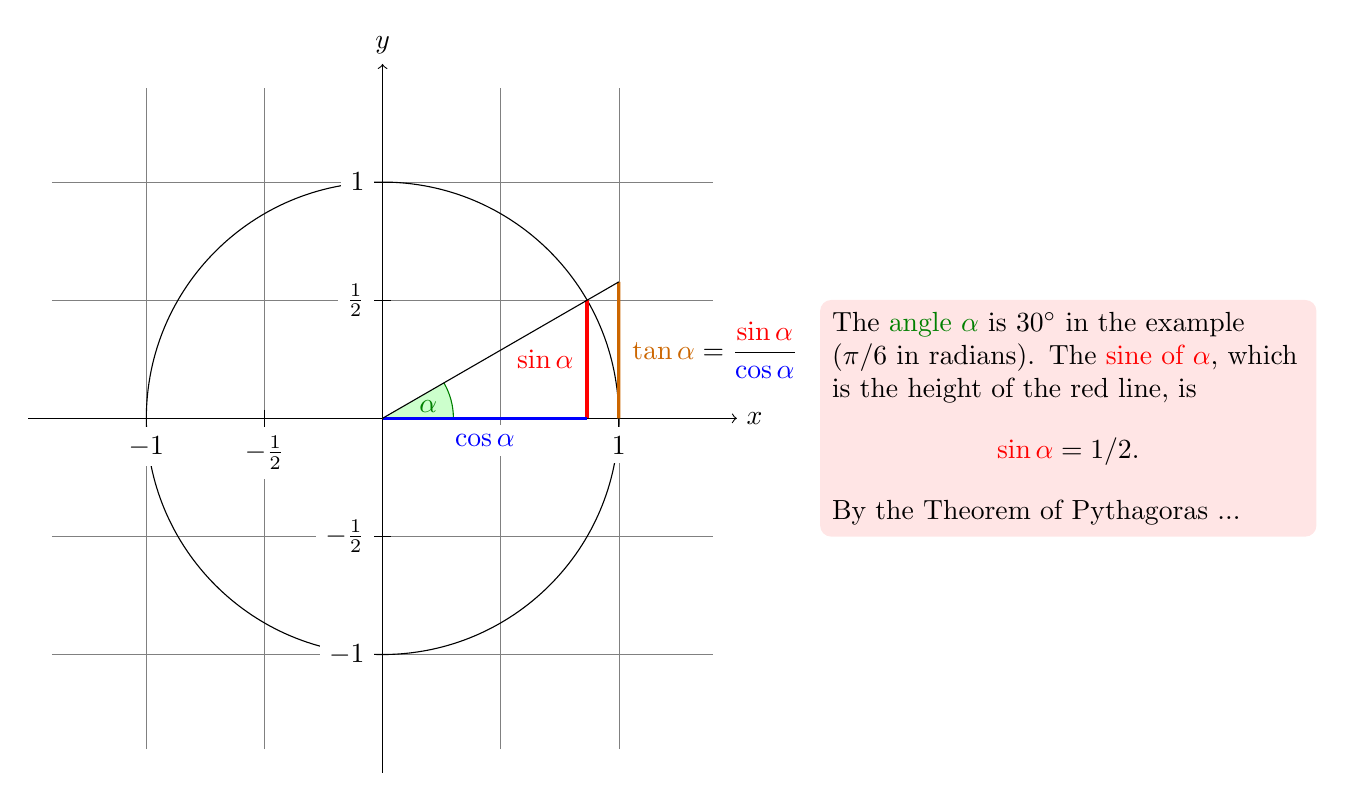
\begin{tikzpicture}
[scale=3,line cap=round
% Styles
axes/.style=,
important line/.style={very thick},
information text/.style={rounded corners,fill=red!10,inner sep=1ex}]
% Local definitions
\def\costhirty{0.8660256}
% Colors
\colorlet{anglecolor}{green!50!black}
\colorlet{sincolor}{red}
\colorlet{tancolor}{orange!80!black}
\colorlet{coscolor}{blue}
% The graphic
\draw[help lines,step=0.5cm] (-1.4,-1.4) grid (1.4,1.4);
\draw (0,0) circle (1cm);
\begin{scope}
\draw[->] (-1.5,0) -- (1.5,0) node[right] {$x$} coordinate(x axis);
\draw[->] (0,-1.5) -- (0,1.5) node[above] {$y$} coordinate(y axis);
\foreach \x/\xtext in {-1, -.5/-\frac{1}{2}, 1}
\draw[xshift=\x cm] (0pt,1pt) -- (0pt,-1pt) node[below,fill=white] {$\xtext$};
\foreach \y/\ytext in {-1, -.5/-\frac{1}{2}, .5/\frac{1}{2}, 1}
\draw[yshift=\y cm] (1pt,0pt) -- (-1pt,0pt) node[left,fill=white] {$\ytext$};
\end{scope}
\filldraw[fill=green!20,draw=anglecolor] (0,0) -- (3mm,0pt) arc(0:30:3mm);
\draw (15:2mm) node[anglecolor] {$\alpha$};
\draw[important line,sincolor]
(30:1cm) -- node[left=1pt,fill=white] {$\sin \alpha$} (30:1cm |- x axis);
\draw[important line,coscolor]
(30:1cm |- x axis) -- node[below=2pt,fill=white] {$\cos \alpha$} (0,0);
\draw[important line,tancolor] (1,0) -- node[right=1pt,fill=white] {
$\displaystyle \tan \alpha \color{black}=
\frac{{\color{sincolor}\sin \alpha}}{\color{coscolor}\cos \alpha}$}
(intersection of 0,0--30:1cm and 1,0--1,1) coordinate (t);
\draw (0,0) -- (t);
\draw[xshift=1.85cm]
node[right,text width=6cm,information text]
{
The {\color{anglecolor} angle $\alpha$} is $30^\circ$ in the
example ($\pi/6$ in radians). The {\color{sincolor}sine of
$\alpha$}, which is the height of the red line, is
\[
{\color{sincolor} \sin \alpha} = 1/2.
\]
By the Theorem of Pythagoras ...
};
\end{tikzpicture}


\begin{tikzpicture}
\path ( 0,2) node [shape=circle,draw] {}
( 0,1) node [shape=circle,draw] {}
( 0,0) node [shape=circle,draw] {}
( 1,1) node [shape=rectangle,draw] {}
(-1,1) node [shape=rectangle,draw] {};
\end{tikzpicture}




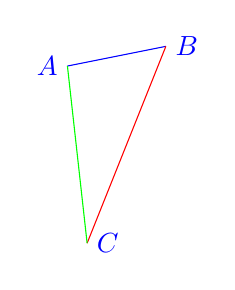
\begin{tikzpicture}
\coordinate [label=left:\textcolor{blue}{$A$}] (A) at (0,0);
\coordinate [label=right:\textcolor{blue}{$B$}] (B) at (1.25,0.25);
\coordinate [label=right:\textcolor{blue}{$C$}] (C) at (0.25,-2.25);
\draw[blue] (A) -- (B);
\draw[red] (C) -- (B);
\draw[green] (A) -- (C);
\end{tikzpicture}

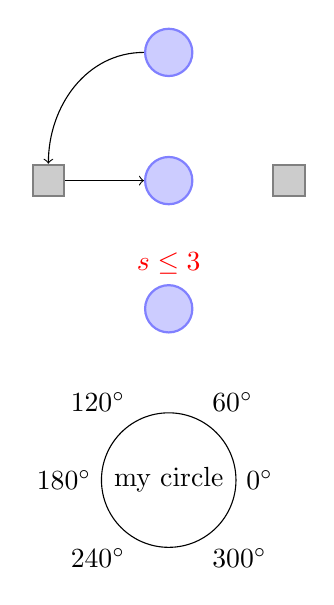
\begin{tikzpicture}
%defines
  [place/.style={circle,draw=blue!50,fill=blue!20,thick,
inner sep=0pt,minimum size=6mm},
transition/.style={rectangle,draw=black!50,fill=black!20,thick,
inner sep=0pt,minimum size=4mm}]
%nodes
\node[place]      (waiting)                            {};
\node[place]      (critical)       [below=of waiting]  {};
\node[place]      (semaphore)      [below=of critical,
                                    label={[red]90:$s\le 3$}] {};
\node[transition] (leave critical) [right=of critical] {};
\node[transition] (enter critical) [left=of critical]  {};
\node [circle,draw,label=0:$0^\circ$,label=60:$60^\circ$,label=180:$180^\circ$,label=240:$240^\circ$,label=120:$120^\circ$,label=300:$300^\circ$]       (newone)      [below=of semaphore] {my circle};
%links
\draw [->] (enter critical) to (critical);
\draw [->] (waiting) to [out=180,in=90] (enter critical);
\end{tikzpicture}

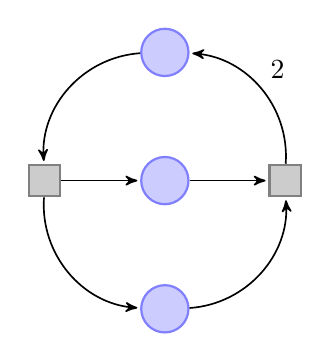
\begin{tikzpicture}
%defines
  [place/.style={circle,draw=blue!50,fill=blue!20,thick,
inner sep=0pt,minimum size=6mm},
transition/.style={rectangle,draw=black!50,fill=black!20,thick,
inner sep=0pt,minimum size=4mm},
bend angle=45,
pre/.style={<-,shorten <=1pt,>=stealth',semithick},
post/.style={->,shorten >=1pt,>=stealth',semithick}]
\node[place] (waiting) {};
\node[place] (critical) [below=of waiting] {};
\node[place] (semaphore) [below=of critical] {};
\node[transition] (leave critical) [right=of critical] {}
edge [pre] (critical)
edge [post,bend right] node[auto,swap] {2} (waiting)
edge [pre, bend left] (semaphore);
\node[transition] (enter critical) [left=of critical] {}
edge [post] (critical)
edge [pre, bend left] (waiting)
edge [post,bend right] (semaphore);
\end{tikzpicture}

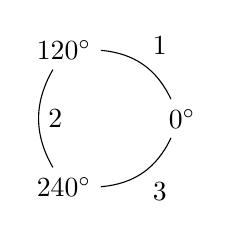
\begin{tikzpicture}[auto,bend right]
\node (a) at (0:1) {$0^\circ$};
\node (b) at (120:1) {$120^\circ$};
\node (c) at (240:1) {$240^\circ$};
\draw 
(a) to node [swap] {1} (b)
(b) to node {2} (c)
(c) to node [swap] {3} (a);
\end{tikzpicture}
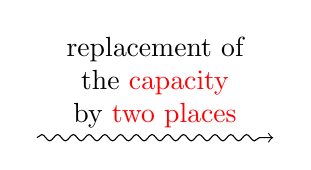
\begin{tikzpicture}
\draw [->,decorate,
decoration={snake,amplitude=.4mm,segment length=2mm,post length=1mm}]
(0,0) -- (3,0)
node [above,text width=3cm,text centered,midway]
{
replacement of the \textcolor{red}{capacity} by
\textcolor{red}{two places}
};
\end{tikzpicture}

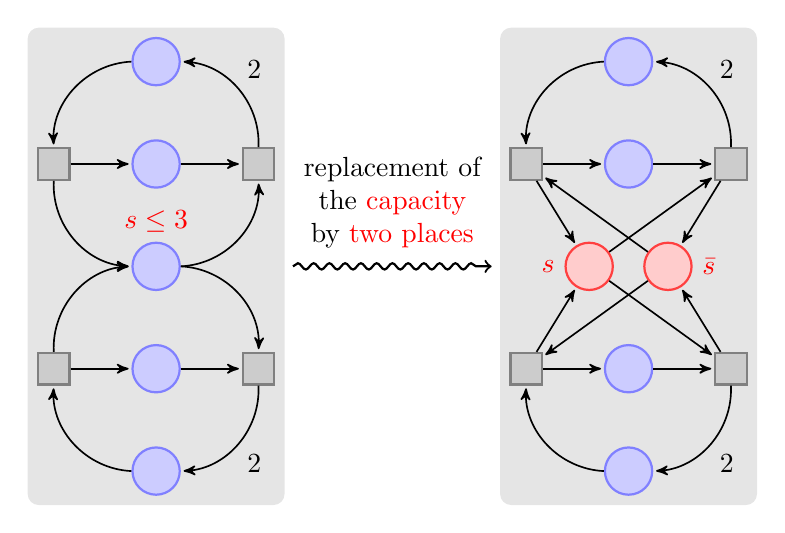
\begin{tikzpicture}
[place/.style={circle,draw=blue!50,fill=blue!20,thick,
inner sep=0pt,minimum size=6mm},
transition/.style={rectangle,draw=black!50,fill=black!20,thick,
inner sep=0pt,minimum size=4mm},
bend angle=45,
pre/.style={<-,shorten <=1pt,>=stealth',semithick},
post/.style={->,shorten >=1pt,>=stealth',semithick},
tokens/.style={},
node distance=1.3cm,on grid,>=stealth',bend angle=45,auto,
every place/.style= {minimum size=6mm,thick,draw=blue!75,fill=blue!20},
every transition/.style={thick,draw=black!75,fill=black!20},
red place/.style= {place,draw=red!75,fill=red!20},
every label/.style= {red}]

\node [place,tokens=1] (w1) {};
\node [place] (c1) [below=of w1] {};
\node [place] (s) [below=of c1,label=above:$s\le 3$] {};
\node [place] (c2) [below=of s] {};
\node [place,tokens=1] (w2) [below=of c2] {};
\node [transition] (e1) [left=of c1] {}
edge [pre,bend left] (w1)
edge [post,bend right] (s)
edge [post] (c1);
\node [transition] (e2) [left=of c2] {}
edge [pre,bend right] (w2)
edge [post,bend left] (s)
edge [post] (c2);
\node [transition] (l1) [right=of c1] {}
edge [pre] (c1)
edge [pre,bend left] (s)
edge [post,bend right] node[swap] {2} (w1);
\node [transition] (l2) [right=of c2] {}
edge [pre] (c2)
edge [pre,bend right] (s)
edge [post,bend left] node {2} (w2);

\begin{scope}[xshift=6cm]
\node [place,tokens=1] (w1') {};
\node [place] (c1') [below=of w1'] {};
\node [red place] (s1') [below=of c1',xshift=-5mm]
[label=left:$s$] {};
\node [red place,tokens=3] (s2') [below=of c1',xshift=5mm]
[label=right:$\bar s$] {};
\node [place] (c2') [below=of s1',xshift=5mm] {};
\node [place,tokens=1] (w2') [below=of c2'] {};
\node [transition] (e1') [left=of c1'] {}
edge [pre,bend left] (w1')
edge [post] (s1')
edge [pre] (s2')
edge [post] (c1');
\node [transition] (e2') [left=of c2'] {}
edge [pre,bend right] (w2')
edge [post] (s1')
edge [pre] (s2')
edge [post] (c2');
\node [transition] (l1') [right=of c1'] {}
edge [pre] (c1')
edge [pre] (s1')
edge [post] (s2')
edge [post,bend right] node[swap] {2} (w1');
\node [transition] (l2') [right=of c2'] {}
edge [pre] (c2')
edge [pre] (s1')
edge [post] (s2')
edge [post,bend left] node {2} (w2');
\end{scope}

\begin{pgfonlayer}{background}
\node (r1) [fill=black!10,rounded corners,fit=(w1)(w2)(e1)(e2)(l1)(l2)] {};
\node (r2) [fill=black!10,rounded corners,fit=(w1')(w2')(e1')(e2')(l1')(l2')] {};
\end{pgfonlayer}
\draw [shorten >=1mm,-to,thick,decorate,
decoration={snake,amplitude=.4mm,segment length=2mm,
pre=moveto,pre length=1mm,post length=2mm}]
(r1) -- (r2) node [above=1mm,midway,text width=3cm,text centered]
{replacement of the \textcolor{red}{capacity} by \textcolor{red}{two places}};
\end{tikzpicture}

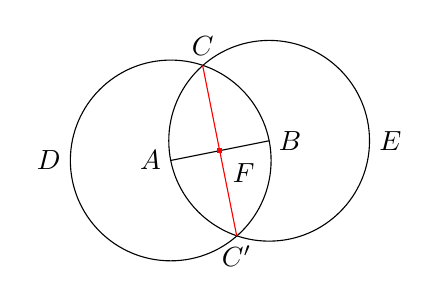
\begin{tikzpicture}
\coordinate [label=left:$A$] (A) at (0,0);
\coordinate [label=right:$B$] (B) at (1.25,0.25);
\draw (A) -- (B);
\node (D) [draw,circle through=(B),label=left:$D$] at (A) {};
\node (E) [draw,circle through=(A),label=right:$E$] at (B) {};
\coordinate [label=above:$C$] (C) at (intersection 2 of D and E);
\coordinate [label=below:$C'$] (C') at (intersection 1 of D and E);
\draw [red] (C) -- (C');
\node [fill=red,inner sep=1pt,label=-45:$F$] (F) at (intersection of C--C' and A--B) {};
\end{tikzpicture}
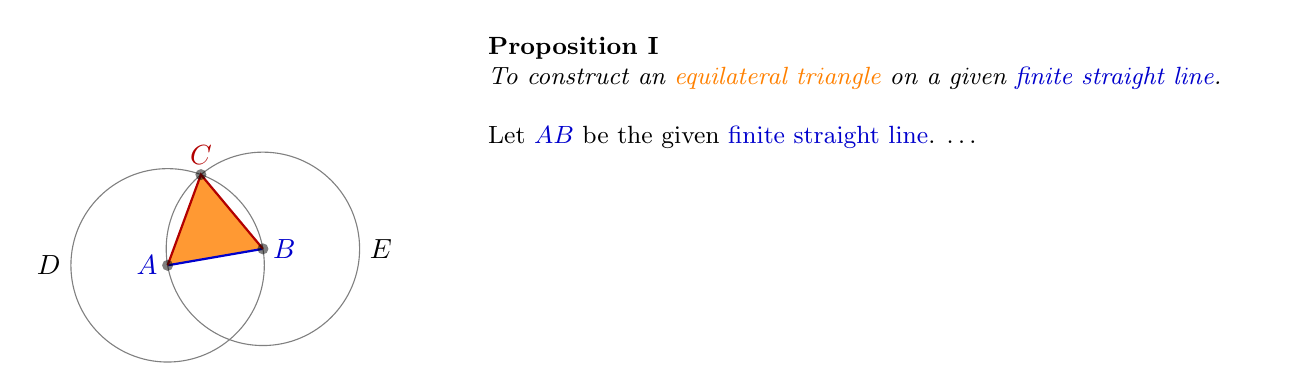
\begin{tikzpicture}[thick,help lines/.style={thin,draw=black!50}]
\def\A{\textcolor{input}{$A$}} \def\B{\textcolor{input}{$B$}}
\def\C{\textcolor{output}{$C$}} \def\D{$D$}
\def\E{$E$}
\colorlet{input}{blue!80!black} \colorlet{output}{red!70!black}
\colorlet{triangle}{orange}
\coordinate [label=left:\A] (A) at ($ (0,0) + .1*(rand,rand) $);
\coordinate [label=right:\B] (B) at ($ (1.25,0.25) + .1*(rand,rand) $);
\draw [input] (A) -- (B);
\node [help lines,draw,label=left:\D] (D) at (A) [circle through=(B)] {};
\node [help lines,draw,label=right:\E] (E) at (B) [circle through=(A)] {};
\coordinate [label=above:\C] (C) at (intersection 2 of D and E);
\draw [output] (A) -- (C) -- (B);
\foreach \point in {A,B,C}
\fill [black,opacity=.5] (\point) circle (2pt);
\begin{pgfonlayer}{background}
\fill[triangle!80] (A) -- (C) -- (B) -- cycle;
\end{pgfonlayer}
\node [below right, text width=10cm,text justified] at (4,3) {
\small\textbf{Proposition I}\par
\emph{To construct an \textcolor{triangle}{equilateral triangle}
on a given \textcolor{input}{finite straight line}.}
\par\vskip1em
Let \A\B\ be the given \textcolor{input}{finite straight line}. \dots
};
\end{tikzpicture}

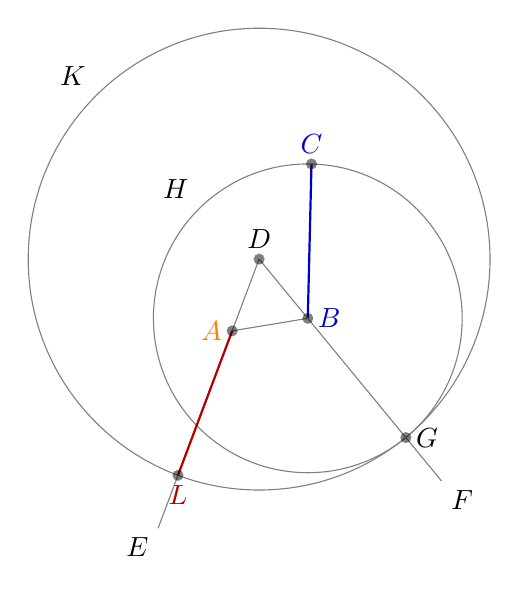
\begin{tikzpicture}[thick,help lines/.style={thin,draw=black!50}]
\def\A{\textcolor{orange}{$A$}} \def\B{\textcolor{input}{$B$}}
\def\C{\textcolor{input}{$C$}} \def\D{$D$}
\def\E{$E$} \def\F{$F$}
\def\G{$G$} \def\H{$H$}
\def\K{$K$} \def\L{\textcolor{output}{$L$}}
\colorlet{input}{blue!80!black} \colorlet{output}{red!70!black}
\coordinate [label=left:\A] (A) at ($ (0,0) + .1*(rand,rand) $);
\coordinate [label=right:\B] (B) at ($ (1,0.2) + .1*(rand,rand) $);
\coordinate [label=above:\C] (C) at ($ (1,2) + .1*(rand,rand) $);
\draw [input] (B) -- (C);
\draw [help lines] (A) -- (B);
\coordinate [label=above:\D] (D) at ($ (A)!.5!(B) ! {sin(60)*2} ! 90:(B) $);
\draw [help lines] (D) -- ($ (D)!3.75!(A) $) coordinate [label=-135:\E] (E);
\draw [help lines] (D) -- ($ (D)!3.75!(B) $) coordinate [label=-45:\F] (F);
\node (H) at (B) [help lines,circle through=(C),draw,label=135:\H] {};
\coordinate [label=right:\G] (G) at (intersection of B--F and H);
\node (K) at (D) [help lines,circle through=(G),draw,label=135:\K] {};
\coordinate [label=below:\L] (L) at (intersection of A--E and K);
\draw [output] (A) -- (L);
\foreach \point in {A,B,C,D,G,L}
\fill [black,opacity=.5] (\point) circle (2pt);
% \node ...
\end{tikzpicture}


\begin{tikzpicture}[
nonterminal/.style={
% The shape:
rectangle,
% The size:
minimum size=6mm,
% The border:
very thick,
draw=red!50!black!50, % 50% red and 50% black,
% and that mixed with 50% white
% The filling:
top color=white, % a shading that is white at the top...
bottom color=red!50!black!20, % and something else at the bottom
% Font
font=\itshape
}]
\node [nonterminal] {unsigned integer};
\end{tikzpicture}

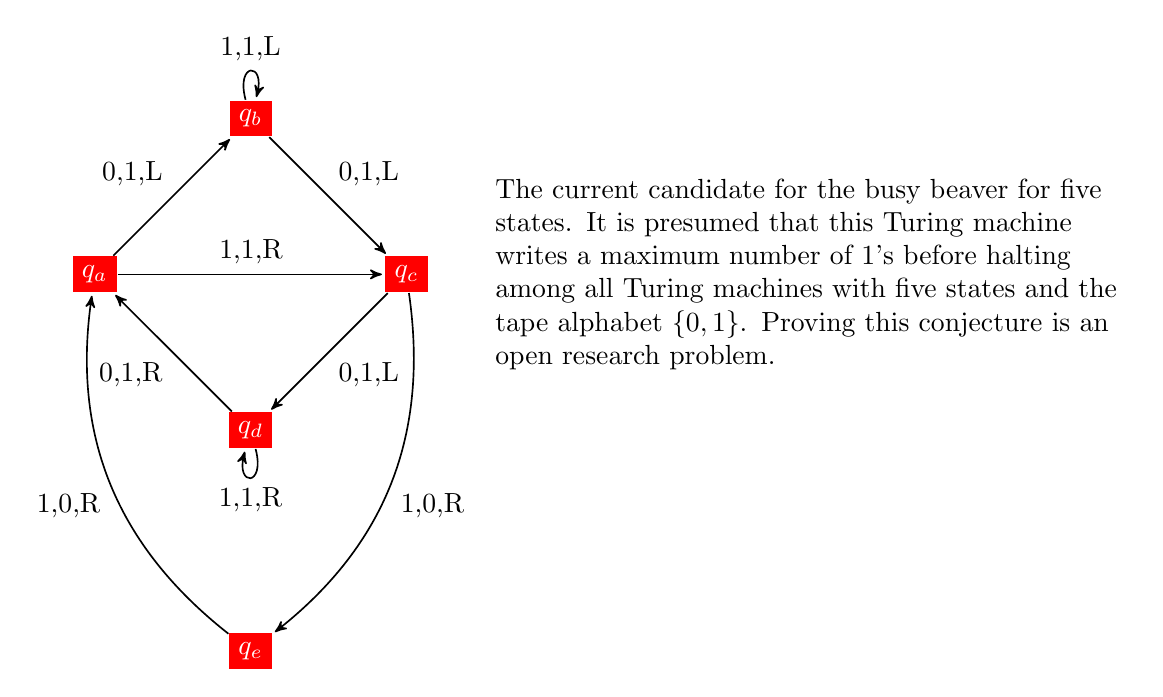
\begin{tikzpicture}[->,>=stealth',shorten >=1pt,auto,node distance=2.8cm,on grid,semithick,
state/.style={fill=red,draw=none,
text=white}]
\node[state] (A) {$q_a$};
\node[state] (B) [above right=of A] {$q_b$};
\node[state] (D) [below right=of A] {$q_d$};
\node[state] (C) [below right=of B] {$q_c$};
\node[state] (E) [below=of D] {$q_e$};
\path (A) edge node {0,1,L} (B)
edge node {1,1,R} (C)
(B) edge [loop above] node {1,1,L} (B)
edge node {0,1,L} (C)
(C) edge node {0,1,L} (D)
edge [bend left] node {1,0,R} (E)
(D) edge [loop below] node {1,1,R} (D)
edge node {0,1,R} (A)
(E) edge [bend left] node {1,0,R} (A);
\node [right=1cm,text width=8cm] at (C)
{
The current candidate for the busy beaver for five states. It is
presumed that this Turing machine writes a maximum number of
$1$'s before halting among all Turing machines with five states
and the tape alphabet $\{0, 1\}$. Proving this conjecture is an
open research problem.
};
\end{tikzpicture}


\par 可用爱因斯坦场方程来表示引力质量其及运动对于周围时空的影响:
\begin{equation}
  \begin{aligned}
  G_{\mu \nu} =R_{\mu \nu} -\frac{1}{2} g_{\mu \nu} R =\frac{8\pi G}{c^4} T_{\mu \nu}
  \end{aligned}
\end{equation}
\par 其中$G_{\mu \nu}$称爱因斯坦张量,$R_{\mu \nu}$为黎曼张量缩并所得的里奇曲率张量,
$R$为空间曲率标量,$g_{\mu \nu}$为四维时空的度规张量,$T_{\mu \nu}$为能量-动量-应力张量,$G$为引力常数。
	对于在纯引力作用下自由运动的一个粒子,根据等效原理,可知存在一个自由降落的坐标系$\xi^\lambda$,
其在这个坐标系中的运动方程是时空中的一条直线,可表示为:
\begin{equation}
    \left\{
    \begin{aligned}
    &0=\frac{d^2 x^\lambda}{d\tau ^2}+\Gamma^\lambda_{\mu \nu}\frac{dx^\mu}{d\tau}\frac{dx^\mu}{d\tau} \\
    &d\tau^2=-g_{\mu\nu}dx^\mu dx^\nu
    \end{aligned}
    \right.
\end{equation}
	其中$\tau$为原时,由度规张量$g_{\mu \nu}$决定;$x^\lambda$,$x^\mu$,$x^\nu$为运动轨迹;
$\Gamma_{\mu \nu}^\lambda$为仿射联络,决定引力场。我们用几何的方式可以把运动方程表述为:
在称为引力场的弯曲时空中一个自由降落的指点将沿着两点间最短可能的路径运动,"长度"由原时来度量的。这样的路径称为测地线。
\section{Method}
\par 为了描述相对论下引力$N$体问题,我们需要引入$N+1$个坐标系:
一个全局坐标系$x^\mu=(ct,x^i)$,
其中包含了所有$N$个引力体并且可以用来描述全局的动力学[1-4];
另外还有$N$个局部坐标系$X^\alpha=(cT_A,X_A^α),A=1,...,N$,这里坐标系$X_A^\alpha$
被假设随天体$A$一起运动。
在本文中,大部分情况下,全局坐标系$\Sigma_glob$指BCRS[5](barycentric celestial reference system,
一个以太阳质心为坐标原点的坐标,适用于整个太阳系范围),
局部坐标系$\Sigma_loc$指GCRS[6](geocentric celestial reference system,
一个以地球质心为坐标原点的坐标,适用于地球附近范围)。
两种坐标系的度规形式假定相同,不同的是势函数,分别为$w^\mu=(w,w^i )与W^\alpha=(W,W^\alpha)$。
进一步假定全局能动张量满足:
\begin{equation}
   \left\{
   \begin{aligned}
   &T^00=O(c^2),T^0i=O(c^(+1)),T^ij=O(c^0) \\
   &\partial_0=\frac{\partial}{\partial ct}=O_1*\partial_i
   \end{aligned}
   \right.
\end{equation}
\par 局部坐标类似。现在可以得到$X^\alpha \rightarrow x^\mu$写成以下形式:
\begin{equation}
  \begin{aligned}
   x^\mu(X^\alpha )=z^\mu (T)+e_\alpha^\mu (T) X^\alpha+\xi^\mu (T,X^\alpha)
  \end{aligned}
\end{equation}
其中$\xi^\mu$至少为$X^\alpha$的二次项,$z^\mu(T)$描述所研究天体上当前选择的点的世界线,
既是该天体的中心世界线,也是天体的后牛顿质心。
\par 引力$N$体问题的全局运动方程来自于局部演化方程
\begin{equation}\label{e:Tensor}
  \begin{aligned}
   T_{\mu;\nu}^\nu=T_{\mu,\nu}^\nu+Γ_\nu\delta^\nu T_\mu^\delta-\Gamma_{\mu\nu}^\delta T_\delta^\nu=0
  \end{aligned}
\end{equation}
式(5)称能量-动量-应力张量的守恒方程,$T_\mu^\nu$称能量-动量-应力张量。
\par 在任何局部系中,局部演化方程(5)在$\mu=0$时取如下形式:~\ref{e:Tensor}
\begin{equation}
  \begin{aligned}
  \frac{\partial}{\partial T} \Sigma + \frac{\partial}{\partial X^a } \Sigma ^a
  =\frac{1}{c^2} \frac{\partial }{\partial T}T^{bb}
  -\frac{1}{c^2} \Sigma \frac{\partial}{\partial T} W+O_4
  \end{aligned}
\end{equation}
在μ=a时取如下形式:
\begin{equation}
  \begin{aligned}
  \frac{\partial}{\partial T} [(1+\frac{4}{c^2}) \Sigma ^a]+
  \frac{\partial}{\partial X^b } (1+\frac{4}{c^2}  W) T^{ab}=F^a+O_4
  \end{aligned}
\end{equation}
其中$\Sigma$,$\Sigma^a$是局部系的能量密度和流,
$F^a=\Sigma E_a+\frac{1}{c^2}  B_{ab} \Sigma^b$。
此式即是后牛顿的欧拉方程。现在固定一天体E(为引力N题系统中一员)的中心世界线,
即$X^a=0$,与后牛顿质心重合$M_a^E (T)=0$,和牛顿力学的情形类似,
现在相应的达朗贝尔原理也会导出引力N体问题中全局平移运动方程。
\section{Conclusion}
\begin{equation}
  \begin{aligned}
 % \begin{multline}
a^{(LD)}_A=&\Sigma_{ B \neq A} \frac{GM_B}{r^2_{AB}}\{1+\frac{1}{c^2}[\nu^2_a+2\nu^2_b-4\nu_A\nu_B-\frac{3}{2}(n_{AB} \cdot \nu_B)^2]\\
&-4 \Sigma_{C \neq A} \frac{GM_C}{c^2r_{AC}}-\Sigma_{C \neq B}\frac{GM_C}{C^2r_{BC}}[1+\frac{1}{2}\frac{r_{AC}}{r_{BC}}n_{AB} \cdot n_{CB}]\}\\
&-\frac{7}{2}\Sigma_{ B \neq A} \Sigma_{ C \neq B}n_{BC}\frac{G^2M_B M_C}{c^2 r_{AB} r_{CB}^2}\\
&+\Sigma_{ B \neq A}(\nu_A-\nu_B)\frac{GM_B}{c^2 r_{AB}}(4 n_{AB} \dot \nu_A- 3 n_{AB} \cdot \nu_B)
 % \end{multline}
  \end{aligned}
\end{equation}
其中:
\begin{equation}
   \left\{
     \begin{aligned}
     &r_{AB}\equiv |z_A(t)-z_B(t)|\\
     &n_{AB}\equiv \frac{z_A(t)-z_B(t)}{r_{AB}}
     \end{aligned}
   \right.
\end{equation}
\par 依据EIH 方程,我们可以用数值方法通过Ruger-Kutta~\cite{Ruger97}计算出 N 体问题引体系统,
如太阳系内的天体运动。
著名的DE历表就是JPL通过EIH计算得到太阳系内大行星运动状态的。
\par 如上文,简要介绍了广义相对论下N个质量单极体运动的一阶近似解,
即多体问题的后牛顿1pN解,
并没有考虑到运动物体的多极距与引电潮汐偶极距。
同时,也有学者研究了后牛顿1.5pN,2.5pN形式及引电潮汐偶极距的影响。
\bibliographystyle{plain}
\bibliography{nbody}
\end{document}